% !TEX root = ../main.tex
% chktex-file 21
\section{Hyperparameter optimization}%
\label{sec:hyperparams}

As described in the introduction, the goal of hyperparameter optimization is to find a global minimum of \(l\).
Since \(l\) is generally unknown, analytical methods or gradient descent cannot usually be applied.
The only way the get information about \(l\) is to evaluate it, which is costly.
There are multiple ways to reduce the total cost of those evaluations:
\begin{enumerate}
	\item \textbf{Number \(T\) of evaluations of \(l\):}
		During optimization multiple hyperparameter configurations \(\lambda_1, \dots, \lambda_T\) will be evaluated using \(l\).
		\(T\) is usually fixed when using a grid search or a random search.
		After evaluating \(T\) configurations, the best one is chosen.
		Those na{\"\i}ve approaches assume that \(l(\lambda)\) is independent of \(l(\lambda')\) for all pairs \(\lambda \neq \lambda'\).
		We will see that this strong assumption of independence is not necessarily true which in turn allows reducing \(T\).
	\item \textbf{Training dataset size \(S\):}
		The performance of a given configuration \(l(\lambda)\) is computed by training the learner on \(\Dtrain\) which is expensive for big datasets.
		By training on \(S\) instead of \(|\Dtrain|\) datapoints the evaluation can be sped up.
	\item \textbf{Number of training iterations \(E\):}
		Depending on the learner, training often is an iterative process, e.~g.\@ gradient descent.
		To speed up hyperparameter optimization training could be terminated before convergence.
\end{enumerate}

\subsection{FABOLAS}%
\label{sec:hyperparams:fabolas}

The first approach we will discuss is called Fabolas (Fast Bayesian Optimization of Machine Learning Hyperparameters on Large Datasets)~\cite{Klein2016}.
It can be applied to any learner \(L\) and is based upon two main ideas:
\begin{enumerate}
	\item The validation loss \(l\) is modeled as a \textit{Gaussian process} (GP) \(f\) based on the assumption that two configurations \(\lambda\) and \(\lambda'\) will perform similar if they are similar according to some kernel \(k(\lambda, \lambda')\).
		The Gaussian process \(f\) is used as a surrogate to estimate the expected value and variance of \(l\) given \(\lambda\).
		Using \textit{Bayesian optimization} \(l\) will be probed at promising positions to iteratively improve \(f\).
		Hyperparameter configurations that are expected to perform worse than the current optimum will not be probed.
		This effectively reduces \(T\).
	\item The training dataset size \(S\) is modeled as an additional hyperparameter of \(f\) giving the optimizer an additional degree of freedom.
		This allows extrapolating the value of \(l\) when trained on the complete dataset while only probing smaller subsets
		which effectively reduces \(S\).
\end{enumerate}
We will now describe how those two ideas can be applied.

\subsubsection{Gaussian processes}%
\label{sec:hyperparams:fabolas:gaussian}

A Gaussian process is a family of \textit{random variables} (RVs) \({(X_\theta)}_{\theta \in \Theta}\), s.~t.\@ every finite subset of them follows a multivariate normal distribution.
More intuitively it can be understood as a probability distribution over functions \(f: \Theta \to \mathbb{R}\) where \(X_\theta \mathrel{\widehat{=}} f(\theta)\).
Prior knowledge about the likelihood of each \(f\) is described by a prior mean function \(\mu_0(\theta) = \mathbb{E}[f(\theta)]\) and a positive-definite kernel \(k(\theta, \theta') = \mathrm{Cov}(f(\theta), f(\theta'))\).
The covariance kernel models how informative it is to know \(f(\theta)\) to determine \(f(\theta')\).

Let \(\mathcal{D}_n = {\{(\bm{\theta}_i, \bm{y}_i)\}}_{i = 1}^{n}\) denote a set of observations.
Those observations can be used to update the means and variances of the RVs via GP regression.
This collapses the space of possible functions \(f\) to those functions that align with \(\mathcal{D}_n\) (see fig.~\ref{fig:fabolas:matern}):
\begin{align}
	\bm{m} :=&\ {(\mu_0(\bm{\theta}_1), \dots, \mu_0(\bm{\theta}_n))}^T \nonumber \\
	\bm{k}(\theta) :=&\ {(k(\bm{\theta}_1, \theta), \dots, k(\bm{\theta}_n, \theta))}^T \nonumber \\
	\bm{K} \in&\ \mathbb{R}^{n \times n}, \bm{K}_{ij} := k(\bm{\theta}_i, \bm{\theta}_j) \nonumber \\
	\mathbb{E}[f(\theta)\, |\, \mathcal{D}_n] :=&\ \mu_n(\theta) = m_0(\theta) + \bm{k}{(\theta)}^T \bm{K}^{-1} (\bm{y} - \bm{m}) \\
	\mathrm{Cov}(f(\theta), f(\theta')\, |\, \mathcal{D}_n) :=&\ k(\theta, \theta') - \bm{k}{(\theta)}^T \bm{K}^{-1} \bm{k}(\theta')
\end{align}

Fabolas works by modeling the loss function \(l\) as a Gaussian process \(f \sim \mathcal{GP}(m, k)\) with parameter set \(\Theta := \Lambda \times [0, 1]\) where \(\mu_0(\lambda, s) = \mathbb{E}[f(\lambda, s)] = \mathbb{E}[l(\lambda)\, |\, \text{training size}\ s]\).
To model the covariances between different combinations of hyperparameters and training set sizes, the following product kernel is used:
\begin{align}
	k((\lambda, s), (\lambda', s')) :=&\ k_{\textsc{Matérn5}}(d_M(\lambda, \lambda')) \cdot k_{\mathrm{lin}}(s, s')
\end{align}
Here \(k_{\textsc{Matérn5}}\) denotes the stationary Matérn kernel (\(\nu = \nicefrac{5}{2}\)) with \(d_M\) being the Mahalanobis distance between the two compared hyperparameter configurations.
\(k_{\mathrm{lin}}\) essentially is a simple linear kernel modeling the assumption that \(l\) monotonically decreases when \(s\) is increased.
We will only give an intuition for this choice of kernel and refer to~\citet{Klein2016} for the details.

The Mahalanobis distance \(d_M\) is used instead of the Euclidean distance because the hyperparameters in a configuration typically use very different scales and are in some cases also correlated.
Figure~\ref{fig:fabolas:mahalanobis} gives an intuition for this.
\begin{figure}[t]
	\centering
	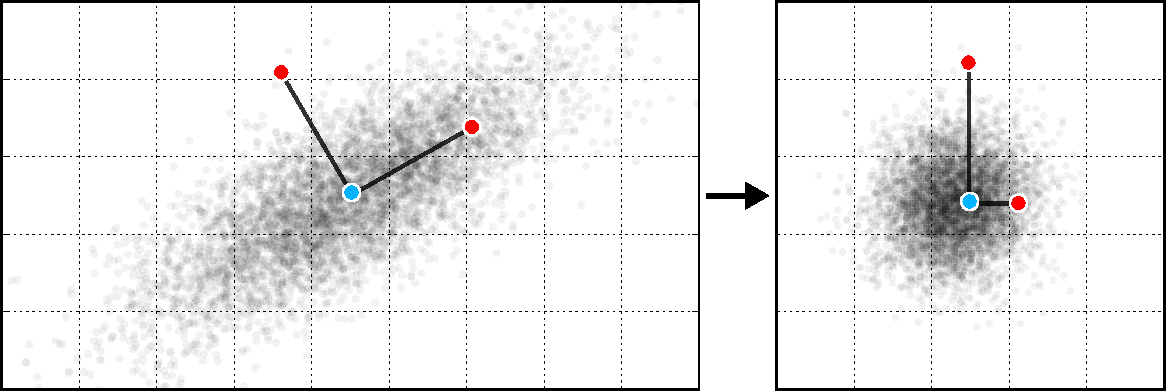
\includegraphics[width=0.7\linewidth]{gfx/fabolas/mahalanobisDistance.pdf}
	\caption{
		Intuition for the Mahalanobis distance.
		Using the Euclidean distance the red points would be equally far away from the blue one.
		The Mahalanobis distance fixes this by first normalizing the hyperparameters and removing correlations.
	}\label{fig:fabolas:mahalanobis}
\end{figure}

Based on the Mahalanobis distance between two configurations \(\lambda, \lambda'\) the \textsc{Matérn5} kernel is used to compute a covariance.
The class of Matérn kernels interpolates between the Gaussian (\textsc{Sq-Exp}) and the exponential (\textsc{Matérn1}) kernel (see fig.~\ref{fig:fabolas:matern}).
Because the exponential kernel drops off quickly, configurations quickly become uncorrelated which causes noisy samples.
The Gaussian kernel drops off less quickly causing smoother samples.
Fabolas uses \textsc{Matérn5} as it empirically fits the smoothness of typical loss functions \(l\) quite well.
\begin{figure}[t]
	\centering
	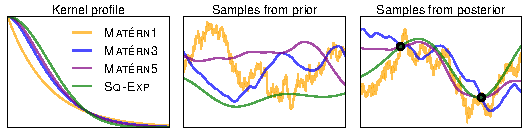
\includegraphics[width=0.75\linewidth]{gfx/fabolas/matern.pdf}
	\caption{
		Comparison between different covariance kernels.
		The middle shows randomly sampled functions \(f\) using different kernels.
		The right shows random samples after two \(f\) values were observed and incorporated into the model via GP regression.
	}\label{fig:fabolas:matern}
\end{figure}

\subsubsection{Bayesian optimization}%
\label{sec:hyperparams:fabolas:bayesian}

To find \(\arg\min_\lambda l(\lambda)\) the bias and variance of \(f\) has to be reduced by probing \(l\) at promising positions.
This is called Bayesian optimization.
The estimated minimum after \(n\) probes is described by \(\arg\min_\lambda \mu_n(\lambda, s = 1)\), i.~e.\@ the configuration with the smallest predicted error on the full test dataset.
To reduce the number of probes required until this minimum converges, an \textit{acquisition function} is used.
Its role is to trade-off exploration vs.\@ exploitation of \(l\) by describing the expected utility of probing \((\lambda_{n+1}, s_{n+1})\) given a set of previous probes \(\mathcal{D}_n\).
Fabolas uses an aquisition function that rates configurations by their \textit{information gain} per computation time:
\begin{align}
	a_F(\lambda, s) :=&\ \frac{1}{c(\lambda, s)} \mathbb{E}_y\left[ p(y\, |\, \lambda, s, \mathcal{D}_n)\ \cdot \mathrm{KL}_{\hat{\lambda}}(p_{\min}(\hat{\lambda}\, |\, \mathcal{D}_n \cup \{(\lambda, s, y)\})\, ||\, u(\hat{\lambda}))\right] \\
	p_{\min}(\lambda\, |\, \mathcal{D}) :=&\ p(\lambda \in \arg\min_{\lambda'}{f(\lambda', s = 1)}\, |\, \mathcal{D}) \nonumber
\end{align}
It measures the expected amount of available information about the optimal configuration if a given configuration were probed, i.~e.\@ the Kullback-Leibler divergence between the density \(p_\min\) of \(\lambda\) being optimal after a probe and the uniform density \(u\).
This information gain of a probe is compared to its expected associated computation time \(c\).
\(c\) is estimated using a separate Gaussian process that is maintained alongside \(f\).
Fabolas considers the cost of a probe because it tries to minimize the total optimization time not the total number of probes.

Since it is infeasible to compute \(a_F\) numerically, its maximum is estimated using \textit{Markov-Chain Monte Carlo} (MCMC).
The estimated most promising configuration will be probed.
The resulting loss value and runtime are then used to update the loss model \(f\) and cost model \(c\) via GP regression.

\subsubsection{Evaluation}%
\label{sec:hyperparams:fabolas:eval}
Fabolas was evaluated in \textit{support vector machine} (SVM) and \textit{convolutional neural network} (CNN) optimization tasks on the MNIST and CIFAR-10 dataset respectively.
Figure~\ref{fig:fabolas:eval} compares Fabolas to the following other hyperparameter optimization approaches:
\begin{itemize}
	\item \textbf{Random Search:}
		Simple random hyperparameter search.
		Each configuration is evaluated on the full dataset.
	\item \textbf{Entropy Search \& Expected Improvement:}
		Bayesian optimization methods that always evaluate on the full dataset.
		Expected Improvement uses an aquisition function that simply probes at the current expected optimum.
		Entropy Search uses an aquisition function similar to the one used by Fabolas but without the cost model.
	\item \textbf{MTBO-\(N\) (Multi-Task Bayesian Optimization):}
		Like Fabolas but restricts probes to two sizes \(s \in \{\nicefrac{1}{N}, 1\}\), i.~e.\@ either a small subsample or the entire dataset is used.
		Multiple values for \(N\) were evaluated: 4, 32 and 512.
\end{itemize}
\begin{figure}
	\begin{subfigure}{0.32\textwidth}
		\centering
		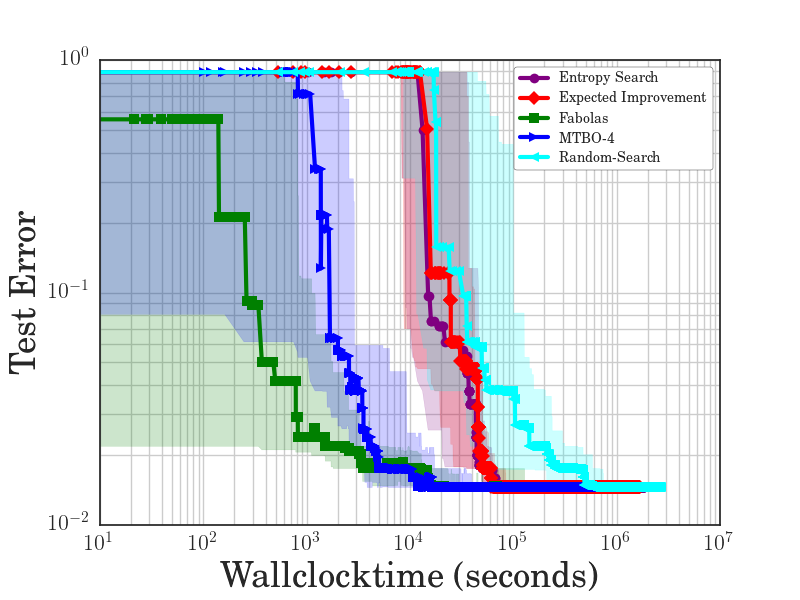
\includegraphics[width=\linewidth]{gfx/fabolas/time1.png}
	\end{subfigure}
	\begin{subfigure}{0.32\textwidth}
		\centering
		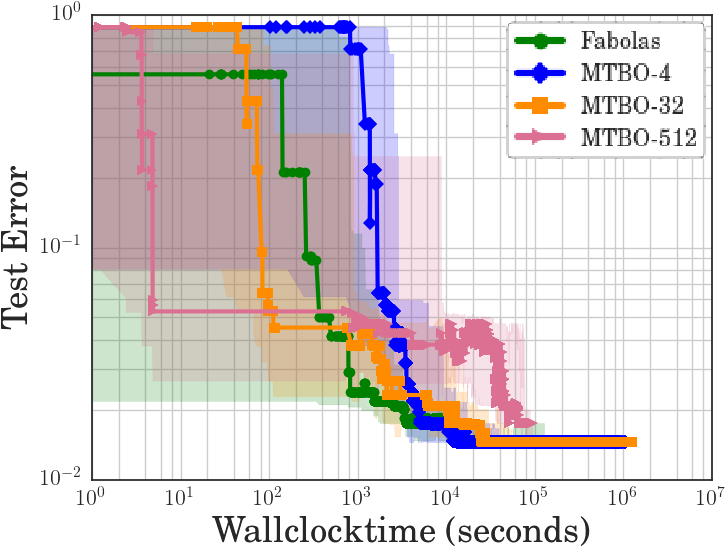
\includegraphics[width=\linewidth]{gfx/fabolas/time2.png}
	\end{subfigure}
	\begin{subfigure}{0.34\textwidth}
		\centering
		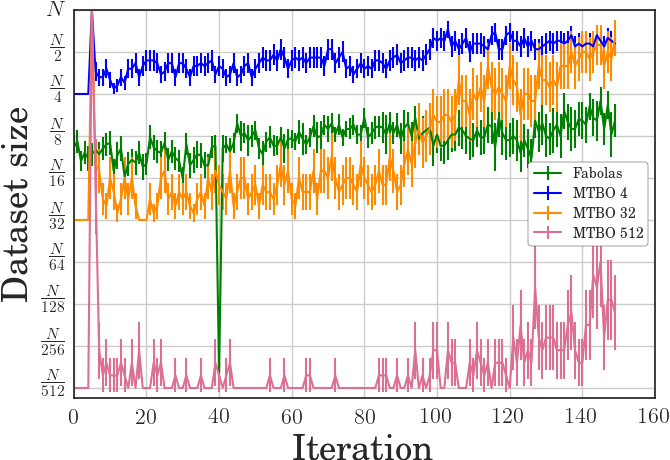
\includegraphics[width=\linewidth]{gfx/fabolas/size.png}
	\end{subfigure}
	\caption{
		SVM optimization on the MNIST dataset.\
		(Left) Comparison of the test performance over time of different optimzers.
		(Middle) Comparison of Fabolas with different MTBO subsample sizes.
		(Right) Comparison of the subsample sizes \(s\) that MTBO and Fabolas choose for their probes.
		The average over 10 runs is depicted.
	}\label{fig:fabolas:eval}
\end{figure}
All Bayesian optimization approaches are at least one order of magnitude faster than random search.
By allowing two probing sizes, MTBO is one additional order of magnitude faster.
Depending on the choice of \(N\) MTBO sometimes improves faster than Fabolas initially.
Once Fabolas starts improving it does however find a good configuration about one order of magnitude faster than MTBO.\
The optimal configuration is found at roughly the same time by both Fabolas and MTBO.\
Overall Fabolas finds a good configuration between 100 and 1000 times faster than random search does.
Similar results are obtained when optimizing CNNs on CIFAR-10.

\subsection{Learning Curve Extrapolation}%
\label{sec:hyperparams:earlyterm}

The second approach for speeding up hyperparameter optimization focuses on reducing the number of training iterations \(E\).
It can in principle be applied to any iterative learner and can be integrated into any hyperparameter optimizer.
The idea is to monitor the learning curve of a learner during training with a hyperparameter configuration \(\lambda\).
If it is unlikely that a good accuracy will be reached with \(\lambda\), training will be terminated before convergence.

The method was first described by \citet{Domhan2015} in the context of hyperparameter optimization for \textit{deep neural networks} (DNNs) that are trained using \textit{stochastic gradient descent} (SGD).

\subsubsection{Extrapolation Method}%
\label{sec:hyperparams:earlyterm:method}

Let \(y_{1:n}\) denote the observed learning curve of SGD after \(n\) iterations, i~e.\@ the sequence of training accuracies \(y_i \in [0, 1]\).
Normally SGD iterations would be run for each hyperparameter configuration \(\lambda\) until convergence or until a maximum number of iterations \(E\) has been reached.
The learning curve extrapolation optimization works by predicting \(y_E\) every \(p\) iterations:
\begin{algorithmic}[1]
\State{\(\hat{y} \gets -\infty\)}
\For{\(\lambda \gets\) next hyperparameter configuration to evaluate}
	\State{\(n \gets 0\)}
	\Repeat\
		\State{Run \(p\) SGD iterations using \(\lambda\) with resulting accuracies \(y_{(n + 1):(n + p)}\).}
		\State{\(n \gets n + p\)}
		\State{Estimate \(P(y_E < \hat{y}\, |\, y_{1:n})\).}\label{line:earlyterm:estimate}
	\Until{\(\text{SGD converged} \lor n \geq E \lor P(y_E < \hat{y}\, |\, y_{1:n}) > \delta\)}
	\State{\algorithmicif\ \(y_n > \hat{y}\) \algorithmicthen\ \(\hat{y} \gets y_n\) \algorithmicend\ \algorithmicif}
\EndFor\
\end{algorithmic}
The prediction step (line~\ref{line:earlyterm:estimate}) uses a probabilistic model.
Similar to Fabolas, a distribution over candidate functions is fit to the observations \(y_{1:n}\).
Unlike Fabolas however, which uses a flexible non-parametric GP model, we use prior knowledge about the shape of learning curves to restrict the model to parameterized, increasing, saturating functions.
More specifically, the learning curve \(y_{1:n}\) is modeled as a linear combination \(f_{\mathit{comb}}\) of a family of given functions.
\begin{align}
	f_{\mathit{comb}}(t\, |\, \xi) :=&\ \sum_{k = 1}^{K} w_k f_k(t\, |\, \theta_k),\
	\xi = (w_1, \dots, w_k, \theta_1, \dots, \theta_k, \sigma^2) \\
	y_t \sim&\ \mathcal{N}(f_{\mathit{comb}}(t\, |\, \xi), \sigma^2)
\end{align}
\citet{Domhan2015} use \(K = 11\) types of functions \(\{f_1, \dots, f_K\}\) that are each parameterized by \(\{\theta_1, \dots, \theta_K\}\).
The assumption is that every function type captures certain aspects of learning curves.
By allowing linear combinations a more powerful model can be obtained.
Figure~\ref{fig:earlyterm:models} illustrates this idea.
\begin{figure}
	\centering
	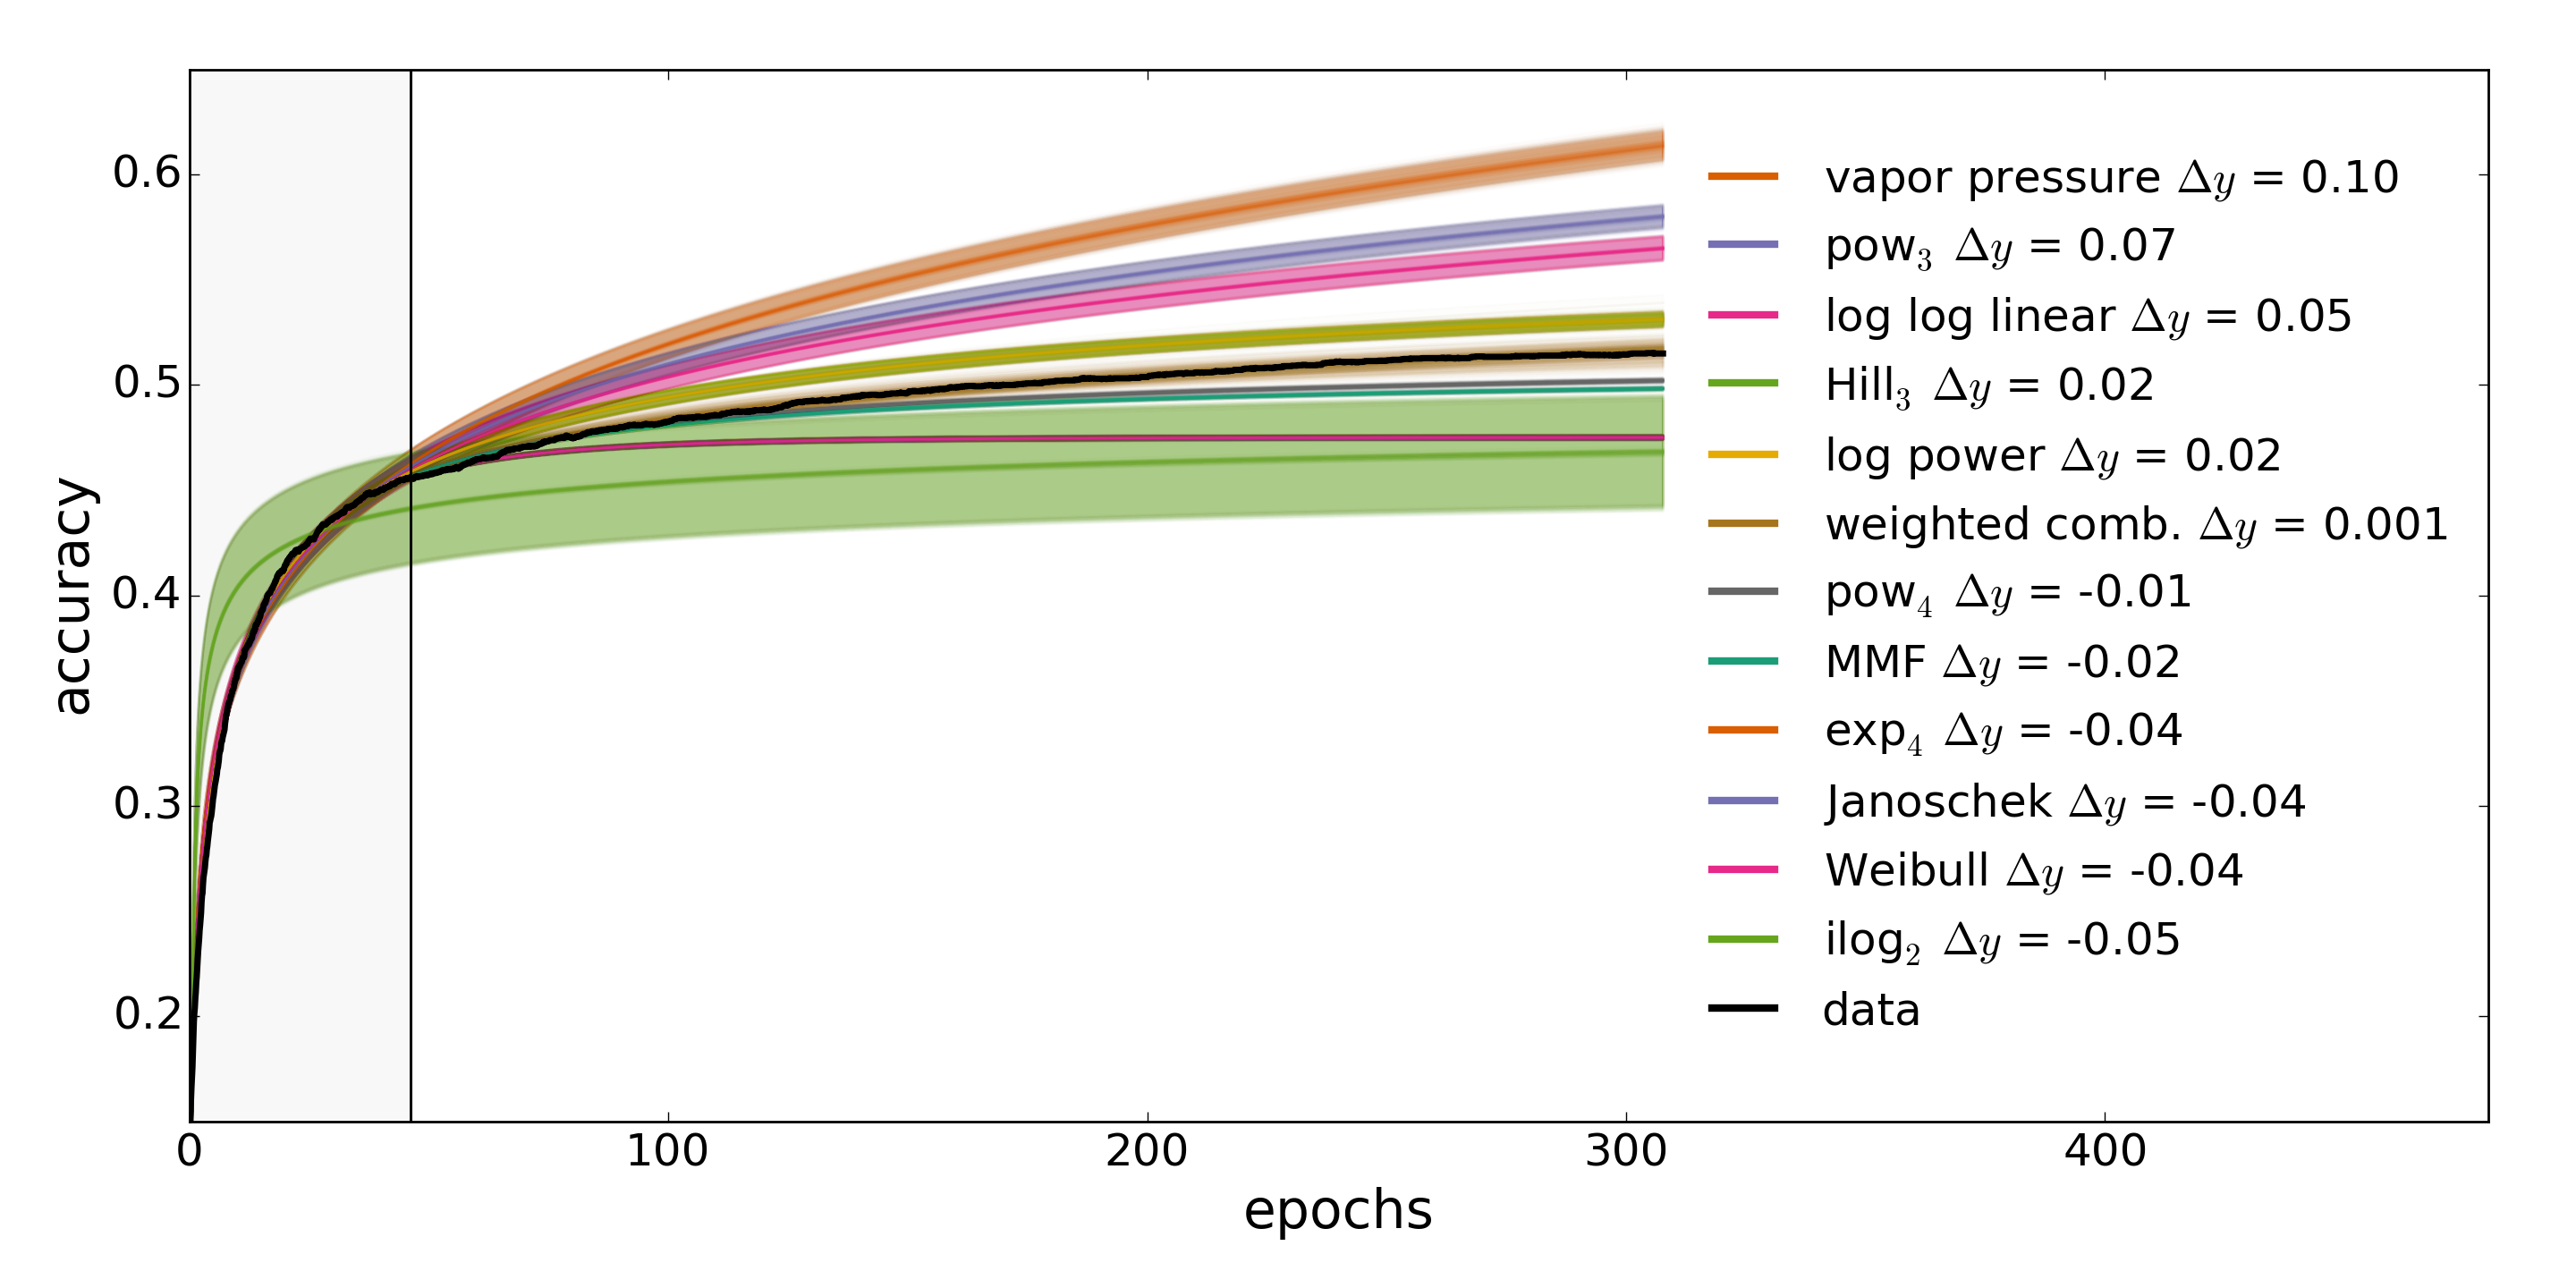
\includegraphics[width=0.75\linewidth]{gfx/earlyterm/models.png}
	\caption{
		Comparison of an observed learning curve (black) with the 11 types of learning curve models and a linear combination of them.
		Each type is parameterized to fit the first 50 observations \(y_{1:50}\).
		As can be seen in the legend on the left, the linear combination has the smallest deviation \(\Delta y\) from the observed data after 300 iterations.
	}\label{fig:earlyterm:models}
\end{figure}
To estimate the probability \(P(y_E < \hat{y}\, |\, y_{1:n})\) MCMC is used to sample \(S\) learning curves \(\{\xi_1, \dots, \xi_S\}\) from the posterior
\begin{align}
	P(\xi\, |\, y_{1:n}) \propto&\ P(y_{1:n}\, |\, \xi) P(\xi) \\
	P(y_{1:n}\, |\, \xi) =&\ \prod_{t = 1}^{n} \mathcal{N}(y_t; f_{\mathit{comb}}(t\, |\, \xi), \sigma^2) \\
	P(\xi) \propto&\ \mathbbm{1}[f_{\mathit{comb}}(1\, |\, \xi) < f_{\mathit{comb}}(E\, |\, \xi) \land \forall k: w_k > 0]
\end{align}
The prior on \(\xi\) is used to model the fact that learning curves do not typically decrease over time.
Given the learning curve samples, we can now estimate
\begin{align}
	P(y_E < \hat{y}\, |\, y_{1:n}) =&\ \int P(\xi\, |\, y_{1:n}) P(y_E < \hat{y}\, |\, \xi)\, \mathrm{d}\xi \\
	\approx&\ \frac{1}{S} \sum_{s = 1}^S \Phi(\hat{y}; f_{\mathit{comb}}(E\, |\, \xi_s), \sigma^2) \nonumber
\end{align}

\subsubsection{Evaluation}%
\label{sec:hyperparams:earlyterm:eval}

The early termination method we just described was evaluated on the CIFAR-10, CIFAR-100 and MNIST dataset.
Figure~\ref{fig:earlyterm:eval} shows the behavior of early termination and the obtained speedup on CIFAR-10.
As expected, configurations with learning curves that tend to approach low accuracies are terminated early.
Configurations with high accuracies are evaluated until convergence.
This approach consistently speeds up the hyperparameter optimization by a factor of two across the tested datasets while reaching the same quality.
\begin{figure}
	\begin{subfigure}{0.4\textwidth}
		\centering
		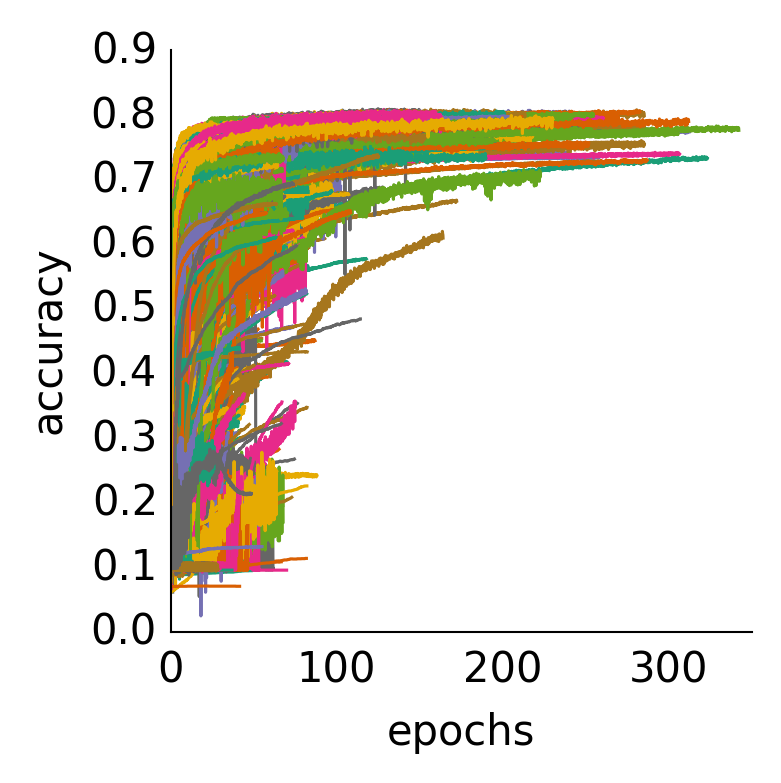
\includegraphics[width=0.9\linewidth]{gfx/earlyterm/samples.png}
	\end{subfigure}
	\begin{subfigure}{0.6\textwidth}
		\centering
		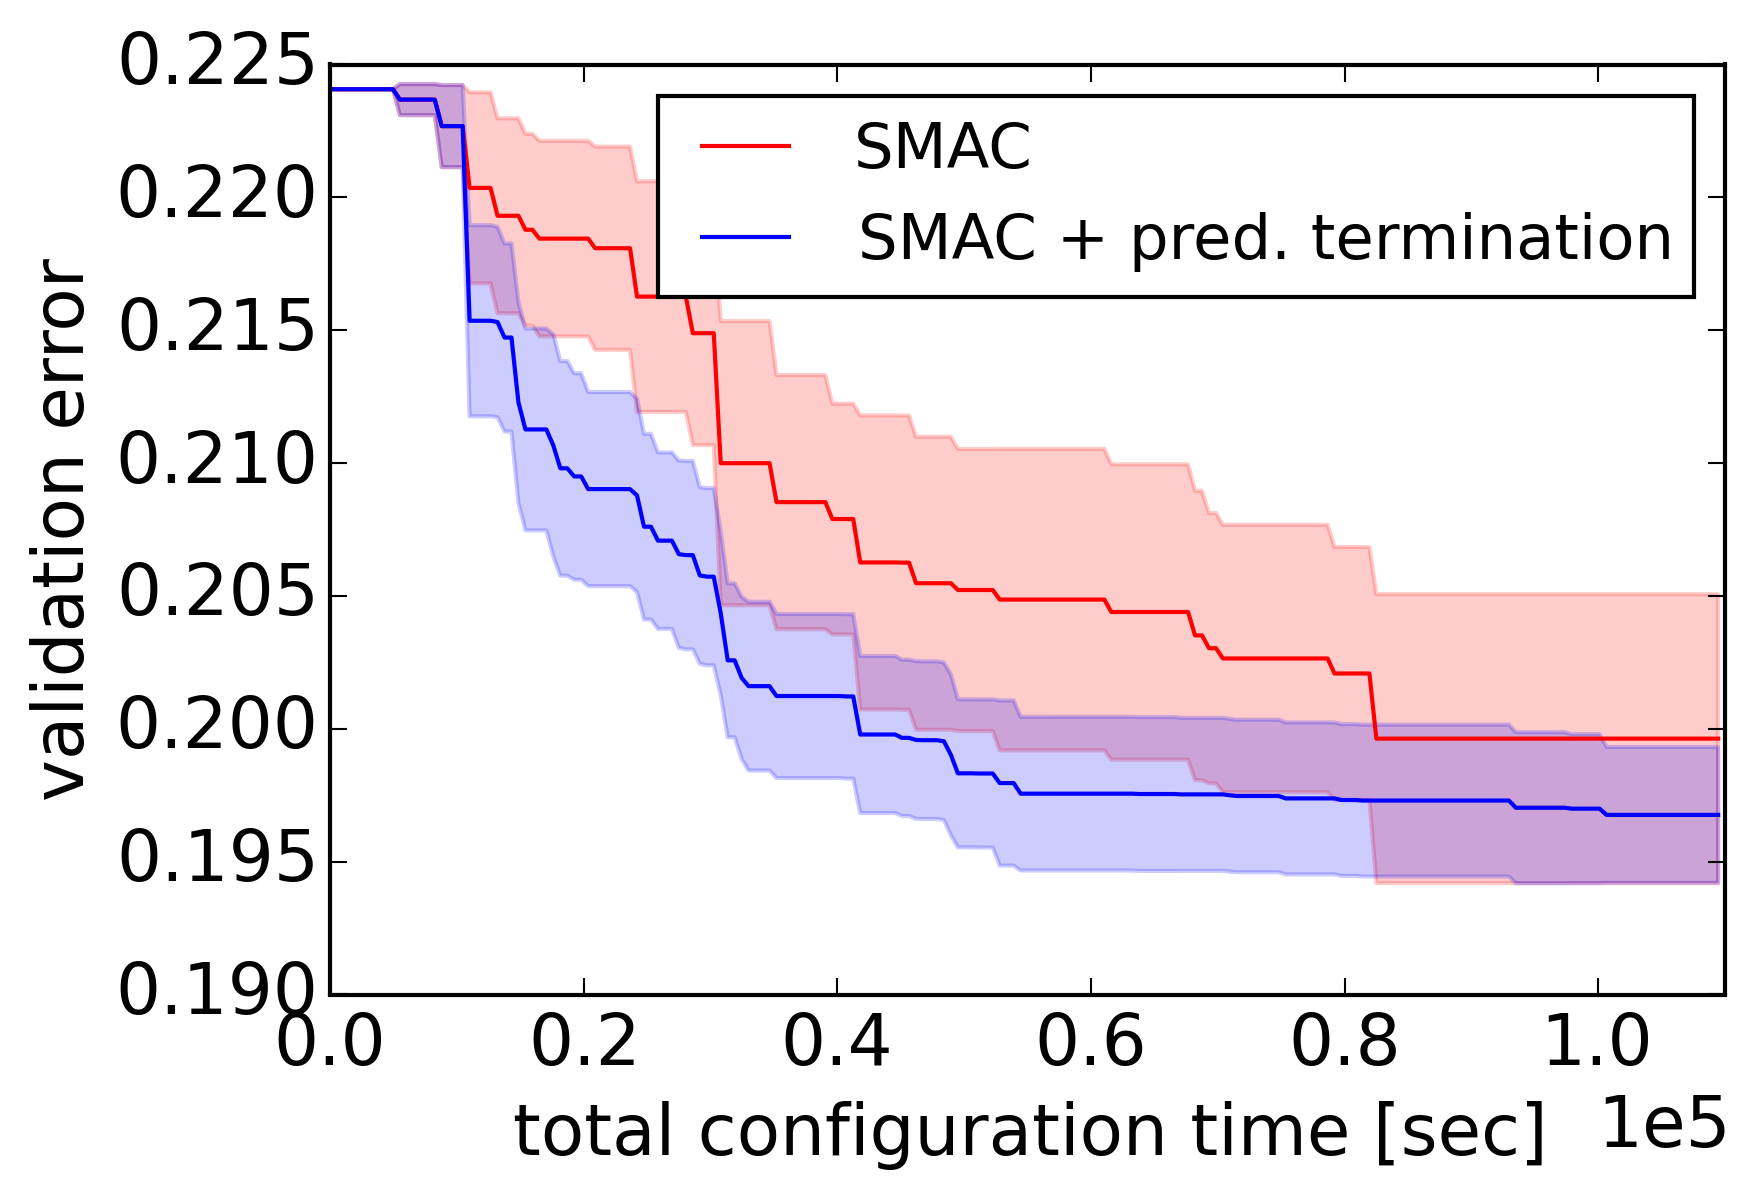
\includegraphics[width=0.8\linewidth]{gfx/earlyterm/time.png}
	\end{subfigure}
	\caption{
		Evaluation on the CIFAR-10 dataset.
		The left graph shows the learning curves of all hyperparameter configurations that were evaluated.
		The right graph shows the average validation error over time.
	}\label{fig:earlyterm:eval}
\end{figure}
